\chapter{Parallel in Time ODE Solver Methods} \label{parareal_chap}
The process of solving time-dependent differential equations in the temporal direction, is an exercise which one would intuitively think is unsuited for parallelization. This is due to the fact that the solution of such equations at every time $T$ depends on the solution at times $t<T$, and it is therefore difficult to partition the solution process into independent tasks that can be solved in parallel. However the Parareal scheme introduced by Lions, Maday and Turinici in \cite{lions2001resolution}is an approach to overcome this limitation. We will however not introduce Parareal as it is described in \cite{lions2001resolution}, but rather present an alternative formulation of the algorithm given in \cite{baffico2002parallel}. Before we state the Parareal algorithm, let us first explain how we decompose the time domain, and an example equation defined on it.
\section{Decomposing the Time Interval} \label{Para_dcomp_sec}
The Parareal scheme is used to parallelize differential equations in temporal direction, by decomposing the time interval $I=[0,T]$. An example of a time-dependent differential equation that on this interval is:
\begin{align}
\left\{
   	\begin{array}{lr}
		\frac{\partial u}{\partial t} + Au = f \ \quad \textrm{for $t \in I$} \\
		u(0)=u_0
	\end{array}
   \right. \label{unbroken}
\end{align} 
Decomposing the interval $I$ means dividing the interval into $N$ subintervals $\{I_i = [T_{i-1},T_{i}]\}_{i=1}^{N}$, with length $\Delta T = T/N$. We define new equations for each interval:
\begin{align}
\left\{
     \begin{array}{lr}
		\frac{\partial u^i}{\partial t} + Au^i = f \ \quad \textrm{for $t \in I^i$} \\
		u^i(T_i)=\lambda_{i-1}
	\end{array}
	\right.	\label{broken}
\end{align}
Here $\lambda_0=u_0$, while $\{\lambda_i\}_{i=1}^{N-1}$ are virtual intermediate initial conditions. If $\Lambda=(\lambda_0,..,\lambda_{N-1})$ are known values, we can solve the equations independently on each interval. The problem is that the $\lambda$'s depend on the solution from previous intervals, and need to be calculated by solving the equation. The Parareal scheme is a way of getting around this.
\section{Parareal}\label{Parareal_sec}
We see that when we decompose the time domain, the original initial value problem (\ref{unbroken}) brakes down to a set of $N$ initial value problems on the form (\ref{broken}). The idea of \cite{baffico2002parallel} is then first to define a fine solution operator $\bold F_{\Delta T}$, which when given an initial condition $\lambda_{i-1}$ at time $T_{i-1}$, evolves $\lambda_i$, using a fine scheme applied to the $i$-th equation (\ref{broken}), from time $T_i$ to $T_{i+1}$. Meaning:
\begin{align*}
\hat \lambda_{i}= u^i(T_{i})=\bold F_{\Delta T}(\lambda_{i-1})
\end{align*} 
We name $\bold F_{\Delta T}$ the fine propagator, and note that letting $\hat \lambda_{1}=\bold F_{\Delta T}(u_0)$, and then applying $\bold F_{\Delta T}$ sequentially to $\hat \lambda_{i}$, is the same as solving (\ref{unbroken}), using the underlying numerical method of the fine propagator. However, we intend to use $\bold F_{\Delta T}$ simultaneously on a given set of initial values $\Lambda=(\lambda_0=u_0,\lambda_1,...,\lambda_{N-1})$, and not sequentially. Since we also want $\hat{\lambda_i}$ to be as close as possible to $\lambda_i$ for $i=1,...,N-1$, we define a coarse propagator $\bold G_{\Delta T}$, and use this operator to predict the $\Lambda$ values. The predictions are made by sequentially applying the coarse propagator to the system (\ref{broken}). This means:
\begin{align}
\lambda_i^0 &= \bold G_{\Delta T}(\lambda_{i-1}^0),\quad i=1,...,N-1, \\
\lambda_0^0&=u_0,
\end{align} 
where the superscript denotes the Parareal iteration. Once we have these predicted initial values, we can apply the fine propagator on all $N$ equations (\ref{broken}) simultaneously, and then use the difference between our fine solution and coarse solution $\delta_{i-1}^0= \bold F_ {\Delta T}( \lambda_{i-1}^0)-\bold G_ {\Delta T}( \lambda_{i-1}^0)$ at time $T_{i}$ to correct $\lambda_i^0$. The correction for time $T_i$, is done by using the coarse propagator on the already corrected $\lambda_{i-1}^1$, and then add the difference $\delta_{i-1}^0$ to $\bold G_ {\Delta T}(\lambda_{i-1}^1)$. When this sequential process is done, we have a new set of initial conditions $\lambda_i^1$, $i=1,...,N-1$, which means that we can redo the correction procedure in an iterative fashion. The prediction-correction formulation of Parareal can then be written up as the following iteration:
\begin{align}
\lambda_{i}^{k+1} &= \bold G_ {\Delta T}(\lambda_{i-1}^{k+1})+\bold F_ {\Delta T}( \lambda_{i-1}^{k})-\bold G_ {\Delta T}( \lambda_{i-1}^{k}), \quad i=1,...,N-1 \label{pred_corr_PR} \\
\lambda_0^k &= u_0
\end{align}
Updating our initial conditions $\Lambda^k$ from iteration $k$ to iteration $k+1$, requires $N$ fine propagations, which we can do in parallel, and $N$ coarse propagations, that we need to do sequentially. We can now write up a simple algorithm for doing $K$ steps of Parareal.
\\
\\
\begin{algorithm}[H]
$\lambda^0_0\leftarrow u_0$\;
\For{$i=1,...,N-1$}{
$\lambda_i^0\leftarrow \bold G_{\Delta T}(\lambda_{i-1}^0)$\;
}
\For{$k=1,...,K$}{
$\lambda_0^k\leftarrow u_0$\;
$\hat{\lambda_{i}^{k}}\leftarrow \bold F_{\Delta T}(\lambda_{i-1}^{k-1})$\tcp*[h]{In parallel}\;
\For{$i=1,...,N-1$}{
$\lambda_i^k\leftarrow \bold G_{\Delta T}(\lambda_{i-1}^k)+\hat{\lambda_{i}^{k}}-\lambda_{i}^{k-1}$\;
}
}
\caption{K steps of the Parareal algorithm\label{P_ALG}}
\end{algorithm}
\noindent
In algorithm \ref{P_ALG} we do $K$ iterations of the Parareal algorithm, where $K$ is a pre-chosen number. If one wanted to construct an actual Parareal algorithm, the iteration should instead terminate, when a certain stopping criteria is met. After $N$ iterations the Parareal algorithm produces the same solution as the fine sequential solver. We therefore need a stopping criteria that ensures that the Parareal solution is sufficiently accurate, while also terminating before $N$ iterations are done. A discussion on suitable stopping criteria for the Parareal algorithm can be found in \cite{lepsa2010efficient}.
\\
\\
Another important component of Parareal, that affects its performance, is the coarse propagator $\bold G_{\Delta T}$. If $\bold F_{\Delta T}$ is based on a finite difference scheme with time step $\Delta t$, one natural choice for $\bold G_{\Delta T}$, would be to use the same scheme as the fine propagator with bigger time step. One must be careful though, since such schemes might be unstable for big time steps. To give an example of a coarse propagator, let us consider a $\bold G_{\Delta T}$ that is based on the implicit Euler scheme with time step $\Delta T$. Using this scheme for our coarse propagator in the context of problem (\ref{unbroken}), would mean that we find $\bold{G}_{\Delta T}(\lambda_i)$ by solving (\ref{G_Backward}) for $\bold{G}_{\Delta T}(\lambda_i)$.
\begin{align}
\frac{\bold{G}_{\Delta T}(\lambda_i) -\lambda_i }{\Delta T } + A \bold{G}_{\Delta T}(\lambda_i) = f(T_{i}) \label{G_Backward}
\end{align}
In the above example we just used a coarse discretization of our problem (\ref{unbroken}) to define the coarse propagator. There are however a lot of other ways to construct $\bold{G}_{\Delta T}$. In \cite{baffico2002parallel} for example, they create the coarse propagator by simplifying the physics of the problem the authors are trying to model. The underlying numerical method of the coarse propagator should in any case be chosen so that the computational cost of $\bold{G}_{\Delta T}$ is negligible in comparison to the cost of  $\bold{F}_{\Delta T}$.
\section{Algebraic Formulation}\label{algebraic_sec}
In \cite{maday2002parareal} an algebraic reformulation of (\ref{pred_corr_PR}) is presented. The setting in \cite{maday2002parareal} is slightly different than the one we had in section \ref{Parareal_sec}, since they are trying to solve an optimal control problem with differential equation constraints, rather than to just solve a differential equation. Luckily for us the problem they are looking at is very much connected to that of solving the time decomposed differential equation system. The problem they solve follows below:
\begin{align*}
&\min_{\Lambda}\hat{J}(\Lambda) = \sum_{i=1}^{N-1} ||u^{i}(T_{i})-\lambda_{i}||^2 \\
&\textrm{Subject to } \ u^{i}(T_{i}) = \bold F_{\Delta T}(\lambda_{i-1}) \ i=1,...,N
\end{align*}
In the above optimal control problem the $\bold F_{\Delta T}$ is the fine propagator from the previous section, and $u$ and $\Lambda$ is also as defined in section \ref{Parareal_sec}. What we immediately notice, is that we can find the solution of the above problem by setting $J(\Lambda)=0$, which gives us the solution $\lambda_{i}= u^{i}(T_{i})=\bold F_{\Delta T}(\lambda_{i-1})$. The authors of \cite{maday2002parareal} then write this system on matrix form as:
\begin{align}
  \left[ \begin{array}{cccc}
   \mathbbold{1} & 0 & \cdots & 0 \\  
   -\bold{F}_{\Delta T} & \mathbbold{1} & 0 & \cdots \\ 
   0 &-\bold{F}_{\Delta T} & \mathbbold{1}  & \cdots \\
   0 &\cdots &-\bold{F}_{\Delta T} & \mathbbold{1}  \\
   \end{array}  \right] 
   \left[ \begin{array}{c}
   \lambda_0 \\
   \lambda_1 \\
   \cdots \\
   \lambda_{N-1} \\
   \end{array}  \right] =
   \left[ \begin{array}{c}
   u_0 \\
   0 \\
   \cdots \\
   0 \\
   \end{array}  \right] \label{vir_mat_form_sys }
\end{align}
Or with notation:
\begin{align}
M \ \Lambda \ = \ H.\quad \textrm{With $M\in\mathbb{R}^{N\times N},H\in\mathbb{R}^N$ given by (\ref{vir_mat_form_sys }).} \label{vir_mat_sys}
\end{align}
We can solve system (\ref{vir_mat_form_sys }) by sequentially applying the fine propagator, but we again want to use the coarse propagator, so that we can run the fine propagator in parallel. We first define the coarse equivalent to $M$ as:
\begin{align}
\bar{M} = \left[ \begin{array}{cccc}
   \mathbbold{1} & 0 & \cdots & 0 \\  
   -\bold{G}_{\Delta T} & \mathbbold{1} & 0 & \cdots \\ 
   0 &-\bold{G}_{\Delta T} & \mathbbold{1}  & \cdots \\
   0 &\cdots &-\bold{G}_{\Delta T} & \mathbbold{1}   \\
   \end{array}  \right]
\end{align}
Using $\bar{M}$, we can write up what turns out to be the Parareal iteration (\ref{pred_corr_PR}) in Matrix notation:
\begin{align}
\Lambda^{k+1} = \Lambda^k + \bar{M}^{-1}(H-M\Lambda^k) \label{matrix_iter1}
\end{align}
Looking at the (\ref{matrix_iter1}), we recognise the Parareal iteration as a preconditioned fix point iteration, where $\bar{M}^{-1}$ is the preconditioner.
\section{Convergence of Parareal}
In this section we look at some of the convergence properties of the Parareal algorithm given in the literature. The first publication on Parareal \cite{lions2001resolution} studied the convergence in context of the following equation: 
\begin{align}
\frac{\partial}{\partial t} y(t)=ay(t),\quad t\in [0,T],\quad y(0)=y_0\label{convergence_ODE}
\end{align}
We state their findings in the proposition below:
\begin{proposition} \label{P_con_prop}
Let us decompose $I=[0,T]$ into $N$ subintervals of length $\Delta T = \frac{T}{N}$, and then let $\bold F_{\Delta T}$ and $\bold G_{\Delta T}$ be the fine and coarse propagators for equation (\ref{convergence_ODE}). If $\bold G_{\Delta T}(\omega)$  is evaluated using the implicit Euler scheme (\ref{G_Backward}), there exist for all integers $k$ a constant $c_k$ such that the error between the $k$-th iterate of the Parareal algorithm (\ref{pred_corr_PR}) and the exact solution of (\ref{convergence_ODE}) $y$ is bounded in the following way:
\begin{align}
\forall \ i,0\leq i\leq N-1 \quad |\lambda_{i}^k-y(T_i)| + \max_{t\in[T_{i},T_{i+1}]}|y_{i+1}^k(t)-y(t)| \leq c_k\Delta T^{k+1} \label{P_error_bound}
\end{align}
\end{proposition}
\noindent
It is important to note that the error bound given in proposition \ref{P_con_prop} only holds for fixed $k$s, since the constant $c_k$ grows with $k$. This means that if we do $k$ iterations of Parareal, the algorithm converges to the  fine numerical solution, when $\Delta T$ goes to zero at a rate of $\mathcal{O}(\Delta T^{k+1})$. We can therefore say that $k$ iterations behaves like a numerical method of order $k+1$. In \cite{lions2001resolution}, the authors used a first order implicit Euler scheme for their coarse propagator. It turns out that if one instead uses a coarse scheme of order $p$, the convergence bound (\ref{P_error_bound}) after $k$ iterations is improved to $\mathcal{O}(\Delta T^{p(k+1)})$. This was shown in \cite{bal2005convergence}, where the bounds were derived for more general equations. 
\\
\\
The case where we let $\Delta T$ be fixed, and look at convergence when we increase $k$, is analysed in \cite{gander2007analysis}. Here the authors again investigate the convergence of the equation (\ref{convergence_ODE}). They found that the convergence was superlinear in $k$ for bounded time intervals $[0,T]$, and linear for unbounded time interval. 
\\
\\
To demonstrate the Parareal algorithm, we will try to verify proposition \ref{P_con_prop} for the following linear ODE:
\begin{align}
\frac{\partial}{\partial t} y(t) =\cos(2\pi t)y(t), \quad t\in[0,4],y(0)=3.52 \label{Parareal_ODE_exs}
\end{align}
This is a simple separable equation with solution $y_e(t)=y_0e^{-\frac{\sin(2\pi t)}{2\pi}}$. To test the Parareal algorithm we choose a fine solver that discretizes (\ref{Parareal_ODE_exs}) using the second order Crank-Nicolson finite difference scheme\cite{crank1947practical}, while we base the coarse solver on a first order implicit Euler scheme. The experimental setup, is to do "zero", one, two and three iterations of Parareal on different time decompositions, and then check if we get the convergence rate proposed in proposition \ref{Parareal_ODE_exs}. The error between the exact solution $y_e$ and the solution $y$ we get from $k$ Parareal iterations is measured in the max-norm, and we use $\Delta t=10^{-6}$ as small time step for the fine discretization. We calculate the convergence rate by comparing the error at different coarse time step sizes $\Delta T_1>\Delta T_2$ using formula:
\begin{align}
\textrm{rate}=\frac{\log(\frac{||y_{\Delta T_2} -y_e||_{l_{\infty}}}{||y_{\Delta T_1}-y_e||_{l_{\infty}}})}{\log(\frac{\Delta T_2}{ \Delta T_2})}. \label{RateDef}
\end{align} 
The results can be found in tables \ref{par_con1} to \ref{par_con4}. Plots of the results of one Parareal iteration applied to large $\Delta T$ values are also added in Figure \ref{P_fig_1_itr}. In table \ref{par_con1} we observe a convergence rate of one, which is in line with proposition \ref{P_con_prop}. For table \ref{par_con2} and \ref{par_con3}, we see that when the coarse time step $\Delta T$ approaches zero, the convergence rate goes to two and three. This is again what we expect in light of proposition \ref{P_con_prop}. In the last table the results are obtained by applying three iterations of Parareal. Proposition \ref{P_con_prop} then suggests a convergence rate of $\mathcal{O}(\Delta T^4)$. We do however not observe this in table \ref{par_con4}, since the error decreases only at a rate of $2.9911$, between $N=1000$ and $N=2000$. The likely cause of this, is that we when doing three iterations of Parareal using $N=1000$ and $N=2000$ approach the underlying error of the fine propagator, and the Parareal algorithm can not outperform the error of the fine scheme.
\\
\\
To illustrate how the Parareal algorithm works, we did a second experiment on equation \ref{Parareal_ODE_exs}. The results of this experiment is presented in figure \ref{P_fig_1_itr}. This figure shows the result of applying one iteration of Parareal to our example problem, using $N=6,12,24$ decompositions of the time interval. We observe that the solution improves when $N$ is increased and consequentially $\Delta T$ is decreased. However, for all decompositions the results are not good, evident by the noticeable jumps between subintervals, and more iterations of Parareal are required to get a satisfactory solution. Another observation about the plots in figure \ref{P_fig_1_itr}, is that the numerical solution is exact (in the sense of the fine scheme) for the two first decomposed intervals. This aspect is especially noticeable for $N=6$. The solution being exact for the $k+1$ first subintervals after $k$ iterations of Parareal is a known property of the algorithm. This property also complicates the implementation of Parareal, since the $k+1$ first processes will become idle after $k$ iterations. Algorithm \ref{P_ALG}, though simple and usable, is not an optimal implementation of Parareal, in part due to the above discussed property.
\\
\begin{table}[h]
\centering
\caption{Results for initial coarse and fine solver applied to equation \ref{Parareal_ODE_exs}. The first column ($N$) represents the number of decomposed subintervals, and the second column is the corresponding coarse time step size $\Delta T=\frac{T}{N}$. The third column measures the maximal absolute difference between the exact solution $y_e$ and the numerical solution $y$ from "zero" steps of Parareal. Using these errors we can find the convergence rate with formula (\ref{RateDef}). We observe a convergence rate of 1, which is as expected for an implicit Euler scheme.}
\label{par_con1}
\begin{tabular}{lrrl}
\toprule
{}$N$ &      $\Delta T$ &       $||y-y_e||_{l_{\infty}}$ &  rate \\
\midrule
40   &  0.100 &  0.802 &       -- \\
50   &  0.090 &  0.628 &  1.09 \\
100  &  0.040 &  0.298 &  1.07 \\
200  &  0.020 &  0.145 &  1.04 \\
500  &  0.008 &  0.057 &  1.01 \\
1000 &  0.004 &  0.028 &  1.00 \\
2000 &  0.002 &  0.014 &  1.00 \\
\bottomrule
\end{tabular}
\end{table}
\begin{table}[h]
\centering
\caption{Convergence results for one iteration of Parareal. The columns are the same as in table \ref{par_con1}. We see a quadratic convergence rate, which is consistent with proposition \ref{P_con_prop}.}
\label{par_con2}
\begin{tabular}{lrrl}
\toprule
{}$N$ &      $\Delta T$ &       $||y-y_e||_{l_{\infty}}$ &     rate \\
\midrule
40   &  0.100 &  3.65e-2 &       -- \\
50   &  0.080 &  2.79e-2 &  1.20 \\
100  &  0.040 &  8.87e-3 &  1.65 \\
200  &  0.020 &  2.42e-3 &  1.87 \\
500  &  0.008 &  4.06e-4 &  1.95 \\
1000 &  0.004 &  1.03e-4 &  1.97 \\
2000 &  0.002 &  2.6e-5 &  1.99 \\
\bottomrule
\end{tabular}
\end{table}
\begin{table}[h]
\centering
\caption{Convergence results for two iterations of Parareal. From proposition \ref{P_con_prop} we expect a convergence rate of three, and we see that the rate of convergence approaches 3 when $\Delta T$ goes to zero.}
\label{par_con3}
\begin{tabular}{lrrl}
\toprule
{}$N$ &      $\Delta T$ &       $||y-y_e||_{l_{\infty}}$ &     rate \\
\midrule
40   &  0.100 &  3.75e-03 &       -- \\
50   &  0.080 &  1.38e-03 &  4.478 \\
100  &  0.040 &  1.09e-04 &   3.66 \\
200  &  0.020 &  2.34e-05 &  2.21 \\
500  &  0.008 &  1.85e-06 &  2.77 \\
1000 &  0.004 &  2.44e-07 &  2.91 \\
2000 &  0.002 &  3.07e-08 &   2.99 \\
\bottomrule
\end{tabular}
\end{table}
\begin{table}[h]
\centering
\caption{Convergence results for three iterations of Parareal. Doing three iterations of Parareal using a first order coarse scheme, we expect that the rate of convergence converges to four. We see that the convergence rate does not behave as we would expect from proposition \ref{P_con_prop}. The most likely explanation for this is that the error of the Parareal algorithm approaches the numerical error of the fine scheme. }
\label{par_con4}
\begin{tabular}{lrrl}
\toprule
{}$N$ &      $\Delta T$ &      $||y-y_e||_{l_{\infty}}$  &     rate \\
\midrule
40   &  0.100 &  2.57e-04 &       -- \\
50   &  0.080 &  7.81e-05 &  5.34 \\
100  &  0.040 &  1.48e-06 &  5.71 \\
200  &  0.020 &  1.34e-07 &  3.46 \\
500  &  0.008 &  6.04e-09 &  3.38 \\
1000 &  0.004 &  4.43e-10 &  3.76 \\
2000 &  0.002 &  5.57e-11 &   2.99 \\
\bottomrule
\end{tabular}
\end{table}
\begin{figure}[h]
\centering
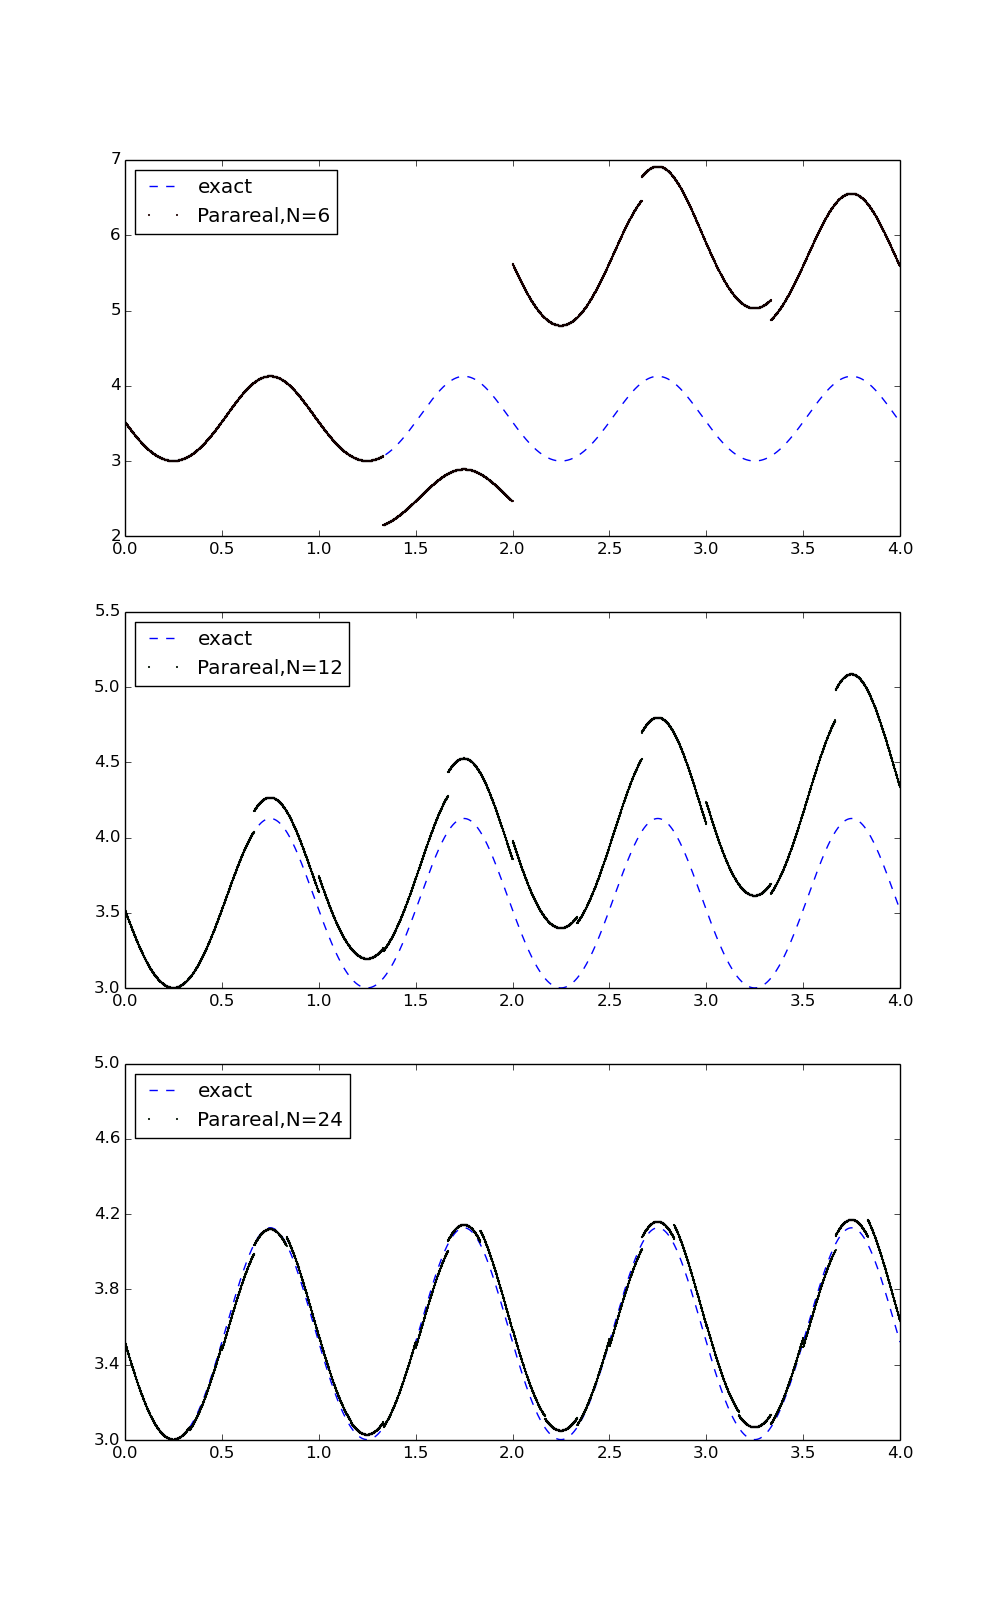
\includegraphics[scale=0.5]{parareal_img.png}
\caption{The result of 1 iteration of the Parareal algorithm on equation (\ref{Parareal_ODE_exs}). The equation is solved using a fine propagator based on the Crank-Nicholsen with resolution $\Delta t=\frac{4}{10^4}$ and a coarse propagator based on implicit Euler. We solve (\ref{Parareal_ODE_exs}) using three different time decompositions, $N=6,12,24$, which translates to coarse time steps $\Delta T=\frac{2}{3},\frac{1}{3},\frac{1}{6}$ used for the coarse propagator. }
\label{P_fig_1_itr}
\end{figure}
